To find a baseline to build upon, we conduct some investigations into the current best methods of Robust Aggregation.
However, aggregators like MKRUM, COMED and FedAvg don't have much complexity to them and as such don't have parameters that can be tuned.
We look into several categories for initial testing such as AFA, FedMGDA+ and aggregator limitations. 
AFA and FedMGDA+ are especially promising in their ability to block faulty/malicious clients. 
It is also important to check how the the local rounds affect detectibility of these bad clients.
\\ \\
In this chapter we assume:
\begin{itemize}
    \item Faulty Clients: 1, 3, 5, 7, 9, 11, 13, 15 17, 19
    \item Malicious Client: 2, 4, 6, 8, 10, 12, 14, 16, 18, 20
    \item Mixed: first 5 of each
\end{itemize}
% Faulty Clients: 1, 3, 5, 7, 9, 11, 13, 15 17, 19
% \\
% Malicious Client: 2, 4, 6, 8, 10, 12, 14, 16, 18, 20
% \\
% Mixed: first 5 of each.
\\
The weighting given to each client as to how much data they get varies from about 2-4\% and is hard-coded in.
\\ \\
One thing to note is that the faulty clients are very faulty in this setup, more broken than just noisy.
This is because just slightly noisy clients can actually benefit the robustness of a model. 
Thus, they are not considered harmful or in need of being detected.

\section{AFA}
For this investigation we kept the local rounds at 10 epochs per round and used all three attacks.
Apart from just looking at the hyper-parameters of xi, deltaxi, aplha and beta, we also observe how many clients get blocked.
This is because one can have a very strict system that ends with good accuracy, but that also blocks a significant number of good clients.
This is not an ideal situation to be in and so should be avoided wherever possible.
We use IID data and are thus less affected, but in real-world situations missing data could have quite a performance impact on the model when testing.

\subsection{Parameters}
\begin{enumerate}
    \item Alpha: the numerator used in calculating the score of each client. Increments if the client doesn't give a bad update. Also used in blocking check via a beta cdf distribution.
    \item Beta: the denominator used in calculating the score of each client. Increments if the client gives a bad update. Also used in blocking check via a beta cdf distribution.
    \item Score: a value used for giving a model weighting in the overall model merging so that we know how much importance to assign each model.
    \item Xi: used as part of calculating whether or not a client should be classified as giving a bad update.
    \item DeltaXi: added the the xi every time there is at least 1 bad update, changing the threshold for being classified as a bad update.
\end{enumerate}
We try a range of xi from one-three, deltaXi from 0.25-0.75 and alpha \& beta from two-four.

\subsection{Results}
The results show:
\begin{enumerate}
    \item 10 malicious clients caused the model to fail in all tests such that it never learned anything regardless of the parameters. [\ref{fig:mal_afa}]
    \item Having a xi value above two causes the initial threshold to be too weak and as such never blocks any clients. This is further shown by when the xi was 2 and the deltaXi was set to 0.75 but to less effect [\ref{fig:afa_2_0.75}]. 
    However, the error rate did wobble and vary a bit between alpha/beta combos and so the model wasn't \textit{completely} destroyed, just not usable.
    \item Lower xi and deltaXi values consistently performed the best and acted more just like a non-federated solution.
\end{enumerate}

It may seem as if the solution is to use a low xi of one or two and a low deltaXi. 
However, we observe that xi values that performed the best and blocked all of the malicious/faulty clients, then proceed to block a hearty amount of benign clients as well.
Around 9-11 of the benign clients get blocked at some point in the training when the xi is one.
\\ \\
This is bad for non-obvious reasons. 
In other aggregators, malicious/faulty clients simply don't get used or receive lower weightings. 
So even if you are a benign client that has some weird data, you can still contribute in some manner or at least aren't branded as bad. 
However, if a hospital gets blocked from contributing more data and isn't allowed access to the finalised model due to a faulty aggregation system, this could negatively impact its ability to provide quality healthcare.
\\ \\
Furthermore, blocking off clients with more unique data may end up harming your model as it only learns the most common data (which can be warped from an attack quite easily!). This is also true in non-IID scenarios.
\\ \\
So we want to find the mix between blocking as few benign clients as possible (ideally none) and blocking as many bad clients as possible (ideally all), while reducing the error rate.
Based on our tests, this leaves us with one option: a xi of two and a deltaXi of 0.25.
This does make sense as we don't want drastic changes each time and so having the delta small at 0.25 works well. 
This is further backed by the best alpha/beta to be both four [\ref{fig:best_afa}] as it then allows for smaller changes in division when calculating the score when the alpha/beta value gets changed.

\begin{figure}[htbp]
	\centering
    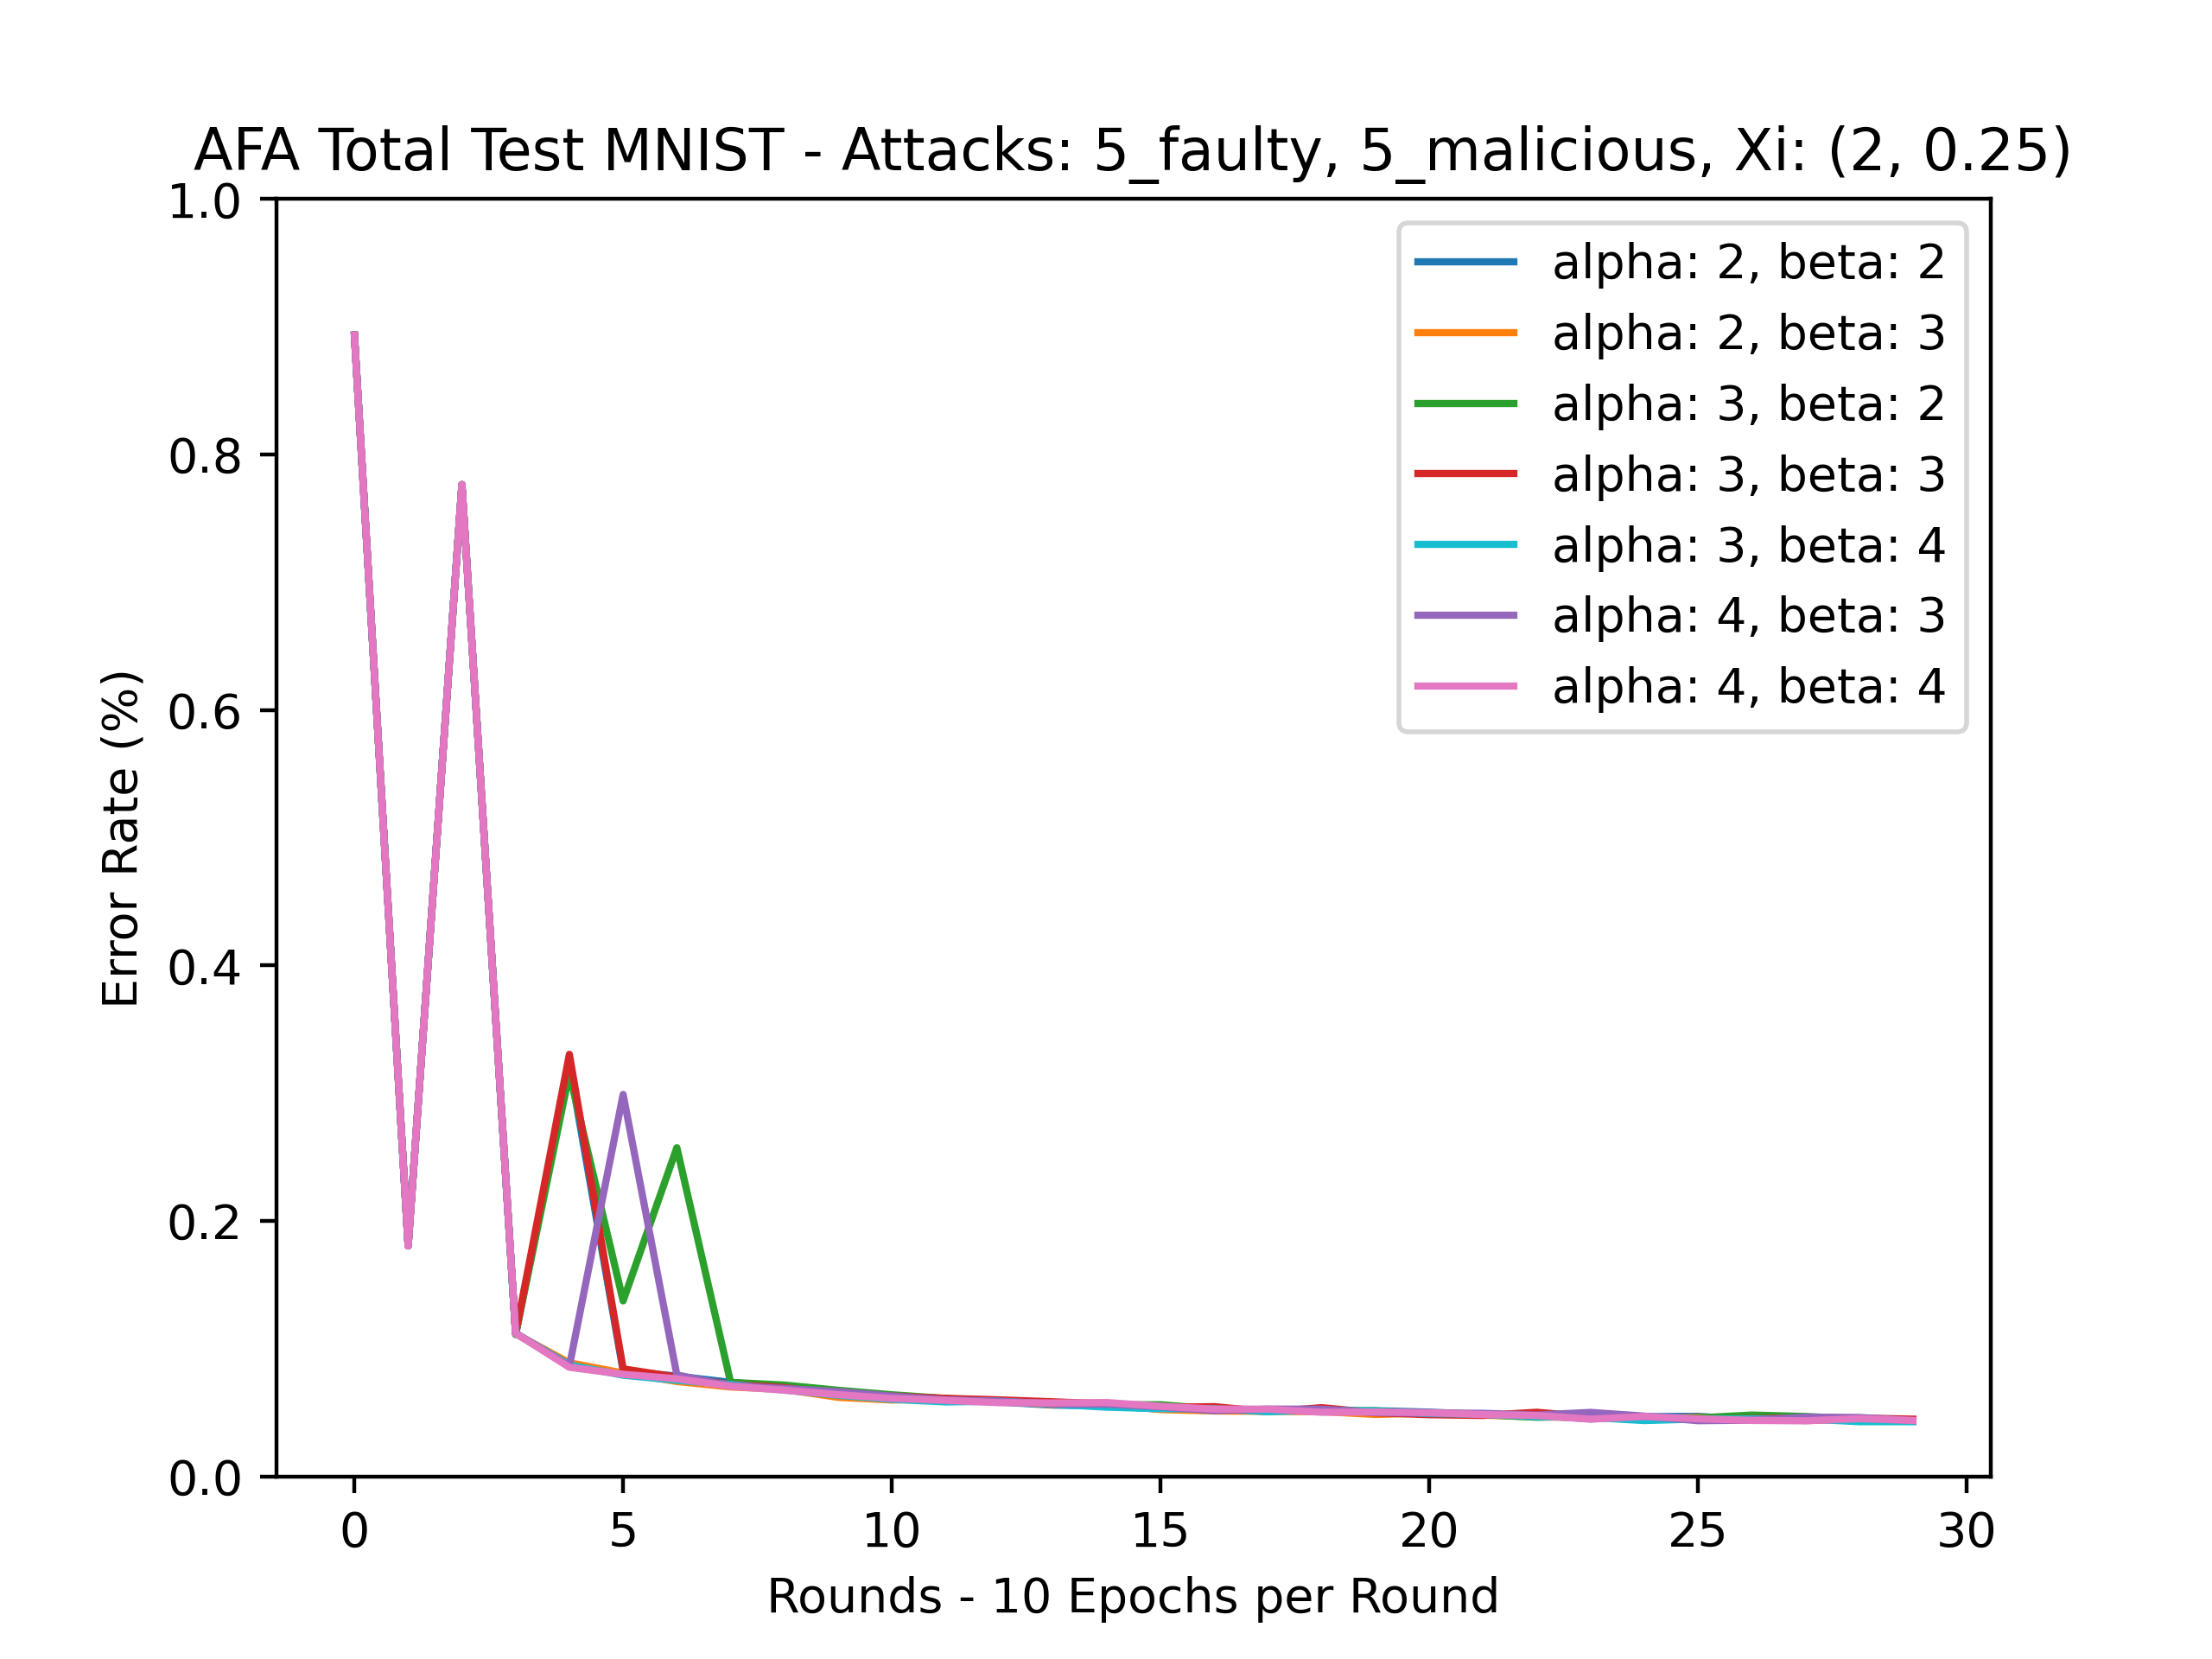
\includegraphics[scale=0.7]{initial/graphs/best_afa.png}
	\caption{AFA - Xi: 2, DeltaXi: 0.25}
	\label{fig:best_afa}
\end{figure}


\section{Improved FedMGDA+}
This investigation was very comprehensive and involved looking at the threshold used for blocking, the LR of the internal layer and the number of epochs per local round. 
Similar investigations were in place to make sure that not too many benign clients were getting blocked for the same reasons labelled above.
For this there were 50 federated rounds with a varying number of epochs per round.
\\ \\
It should be noted that we made significant fixes and improvements to the initial implementation, to ensure its correctness. Ensuring the stability of Improved FedMGDA+ formed a significant portion of our project.

\subsection{Threshold}
Using threshold that are based on a factor inverse to the number of clients involved proved fruitless.
The idea was that if each client had an initial normalised weight of 1/30 (for 30 clients), then having the threshold be 1/60 or 1/300 would mean that the algorithm could handle varying numbers of clients much more easily.
\\ \\
However, all we saw happen is that when the model identified clients as bad, their weights very heavily just went into the negative.
This meant that no manner of factor-based threshold was going to have an impact as the weights would simply hop into the negative.
There were some \textit{slight} deviations as shown in Figure \ref{fig:mgda_var}:
\begin{figure}[htbp]
	\centering
    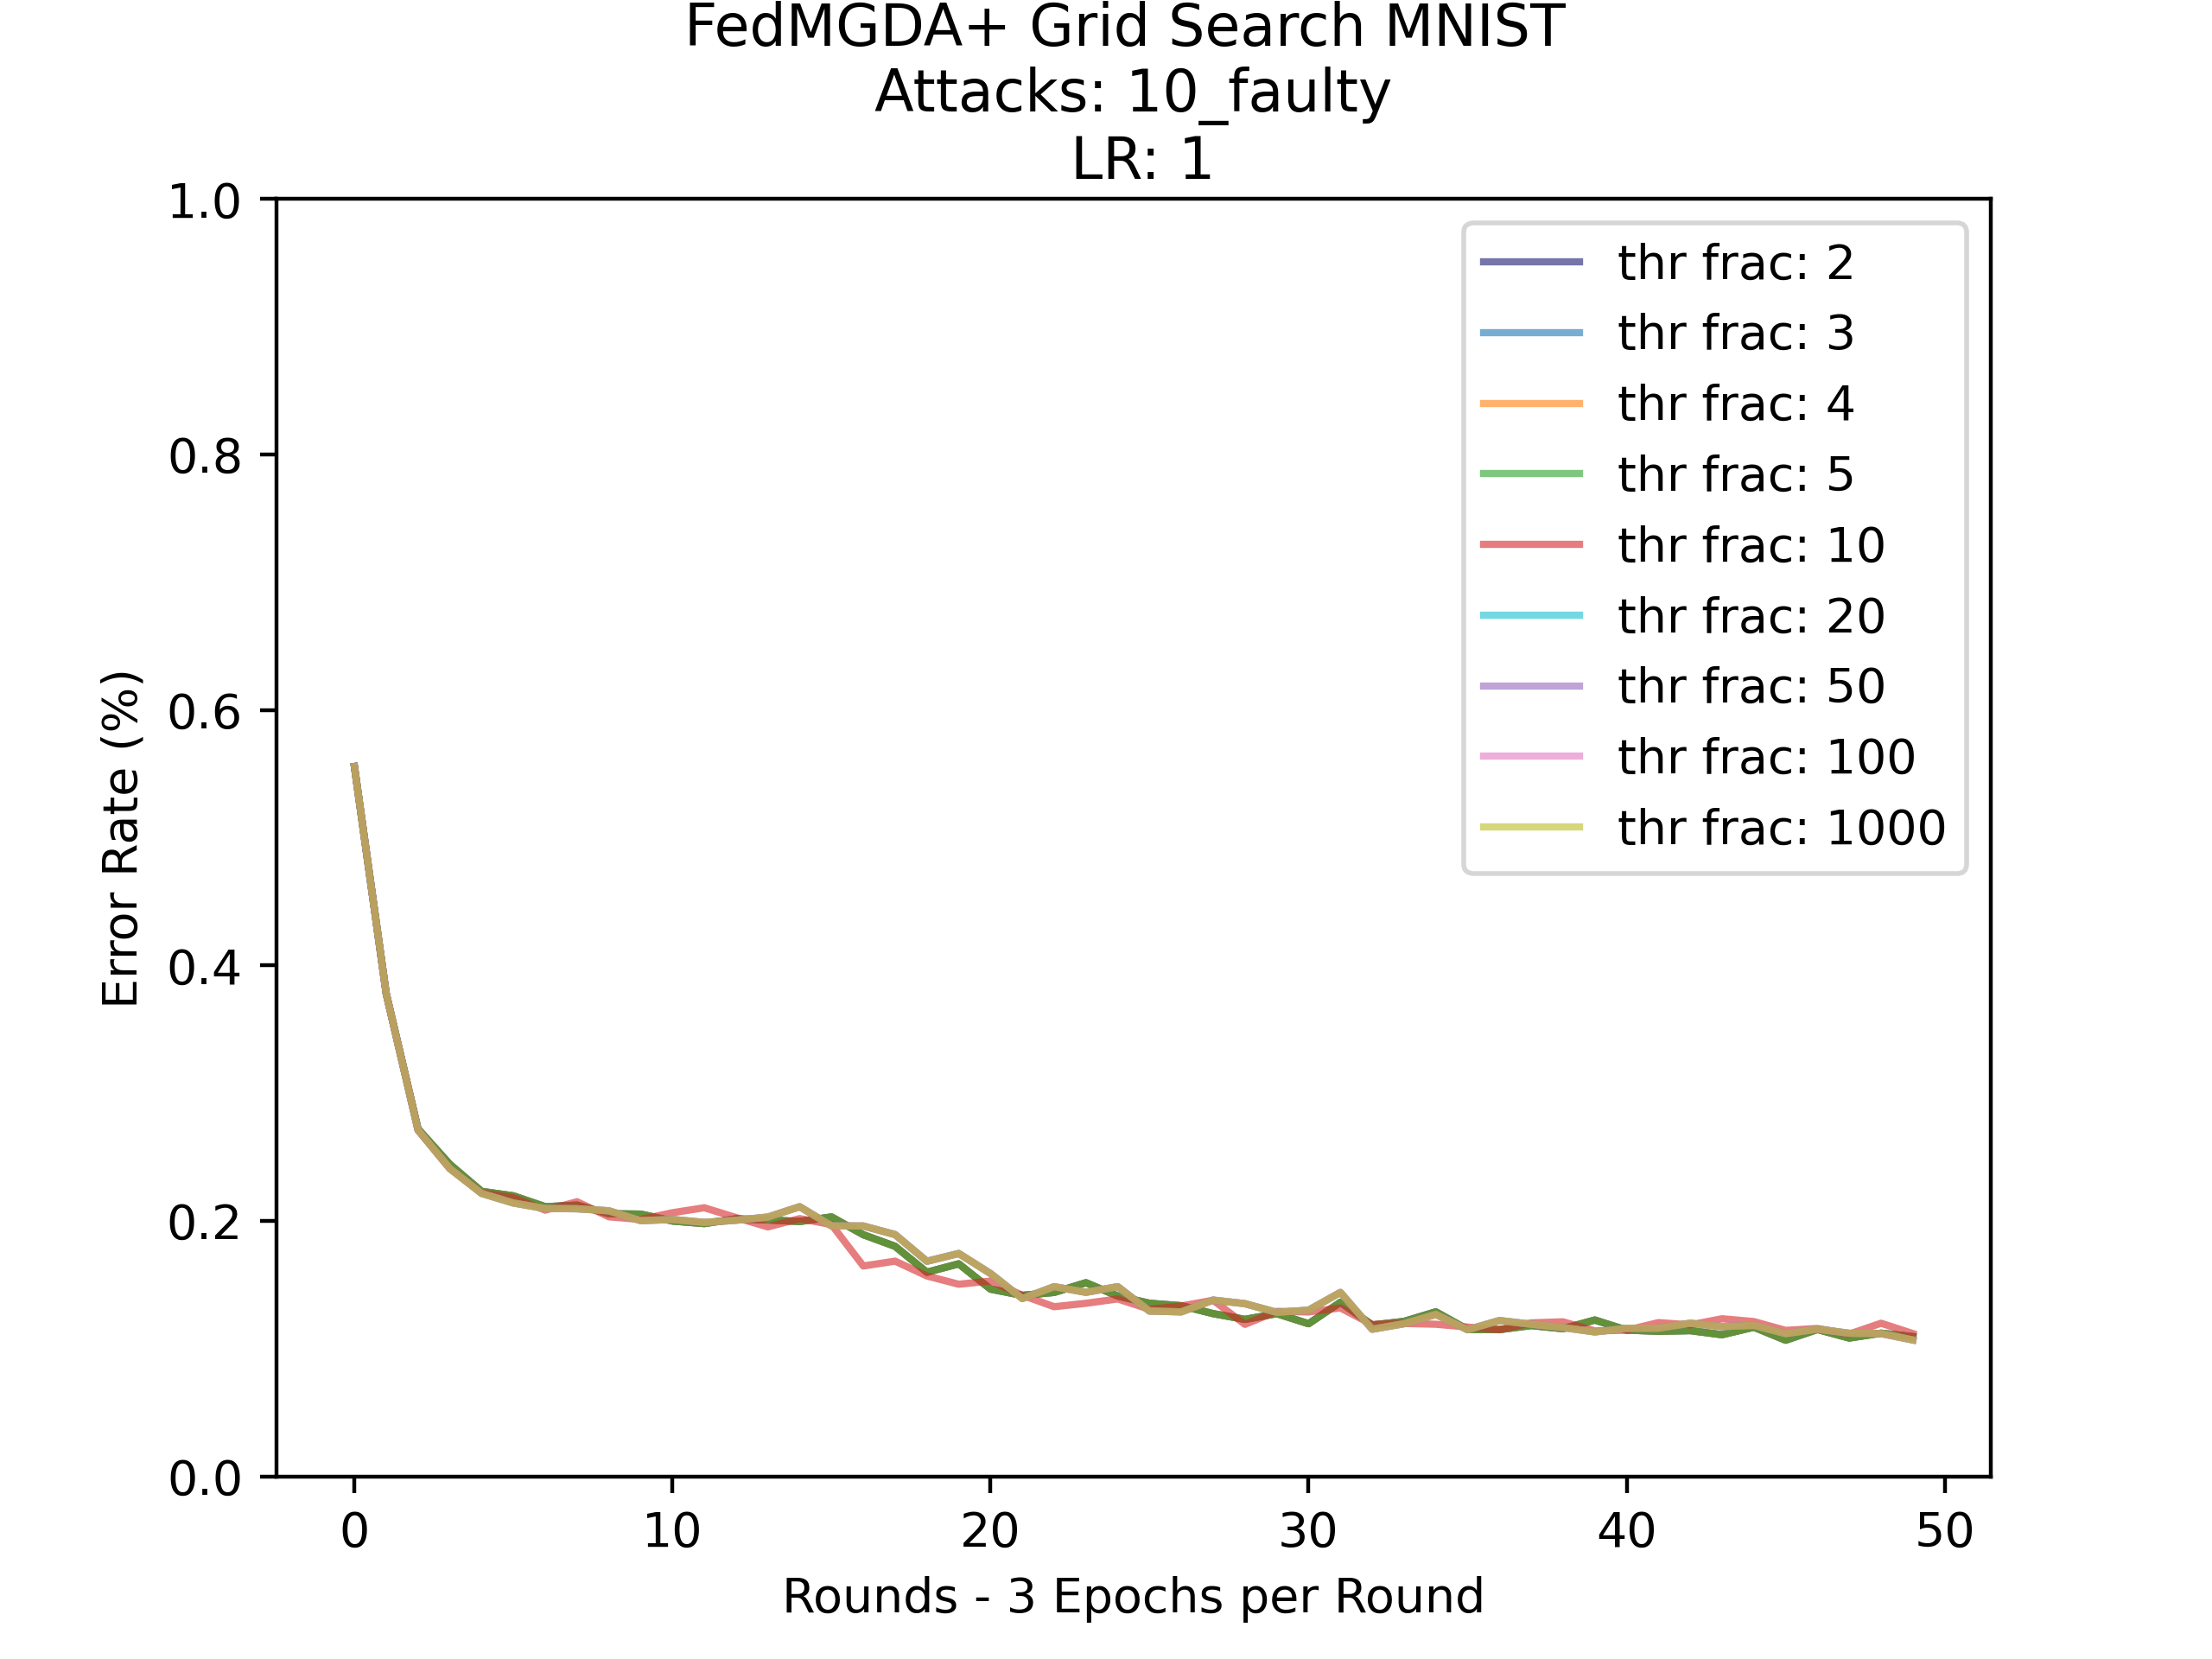
\includegraphics[scale=0.7]{initial/graphs/mgda_var.png}
	\caption{FedMGDA+ Threshold Variance Demo}
	\label{fig:mgda_var}
\end{figure}

\subsection{LR and Epochs}
These two are linked by their relationship; if you increase the number of local epochs per federated round, then overall there will be more rounds of learning going on. 
This also causes the local models to learn more about their own local data before aggregating together. 
This might mean that you might/might not want a higher LR to have the newer parameters taken more seriously.
\\ \\
Looking into the results it is really easy to get tricked and believe that the best option is to just crank up the LR and have at least six local epochs per round. 
This is because you get some great graphs that have the error rate quickly converge to a low result [\ref{fig:fake_good}].
It's noticeable that the LRs above 0.5 have essentially converged by round 10 to a good result.

\subsubsection{Hidden in the Grit}

Alas, just like with AFA, the real information comes out in the grit of which clients were blocked and when.
When you look at that, you see that all-bar-one benign client gets blocked in rounds one-three.
Funnily enough, over these three rounds is exactly when all of the malicious clients get blocked as well.
This pretty much leads me to believe that the malicious clients aren't getting blocked because they are actually being recognised as bad, but instead because the aggregator is deciding to block the clients en-mass.
It just so happens that the malicious ones are caught in the cross-fire of all of the mass blocking.
\\ \\
However, when we look at the lower end of the LR, we get much slower convergence but with absolutely no benign clients being blocked and all of the byzantine ones getting blocked.
This would be cause for celebration if it wasn't taking the aggregator 46 rounds out of 50 to actual do the blocking...
So, looking at lower numbers of epochs per round, we see that 1/2 looked like they work much better.
They showed a mix of being able to block all of the malicious clients [\ref{fig:1epoch_grid}] and achieving a good, low error rate [\ref{fig:2epoch_grid}] but not quite both.
These results tend to occur at around LRs of 0.01 to 0.05 and so further refinement needs to be done.

\subsubsection{Refinement Needed}
Looking into a more refined LR, we again notice that an epoch count of one produces results such that the malicious clients get blocked at great points such a round 16 or so but still don't converge to the ideal error rate.
However, two does not block early enough or ends up blocking some benign clients.
The latter ends up being quite an easy fix as these clients end up being blocked in around the 30\textsuperscript{th}-50\textsuperscript{th} round.
The solution is to reduce the number of rounds that the aggregator runs for.
\\ \\
Finding the balance between these two options proved to be fairly simple: an epoch count of one simply never showed a low enough error rate so two will be the best starting point.
In our project, we use an adaptive approach, and had the LR either increase or decrease as the rounds go on. 
While we could have tried many LR update methods, such as a sinusoidal LR or one that increases and decreases, finding an optimal method would have introduced runaway complexity.
\\ \\ 
A decreasing LR from the values of [0.1, 0.09, 0.08, 0.07, 0.06, 0.05] to [0.05, 0.04, 0.03, 0.02, 0.01] in a linear fashion proved to be the best course of action.
This followed a fairly logical course of thought, such that you want to start out with a higher LR initially to help differentiate between the clients more.
Later on you would then become more certain that the clients should be benign and so you don't need as high of a LR.
However, starting too high (\textgreater0.08) proved fruitless and ending too low just gave results that blocked clients later and later.
The perfect balance here was around from a starting LR of 0.07 and ending up at 0.02 [\ref{fig:best_fedmgda+}], which caused the malicious clients to be blocked at around rounds 11-13.
We also did some experiments with increasing LRs but not only did that follow less of a logical course of action, it subsequently did not provide any benefit or particularly good/useful results.

\begin{figure}[htbp]
    \centering
    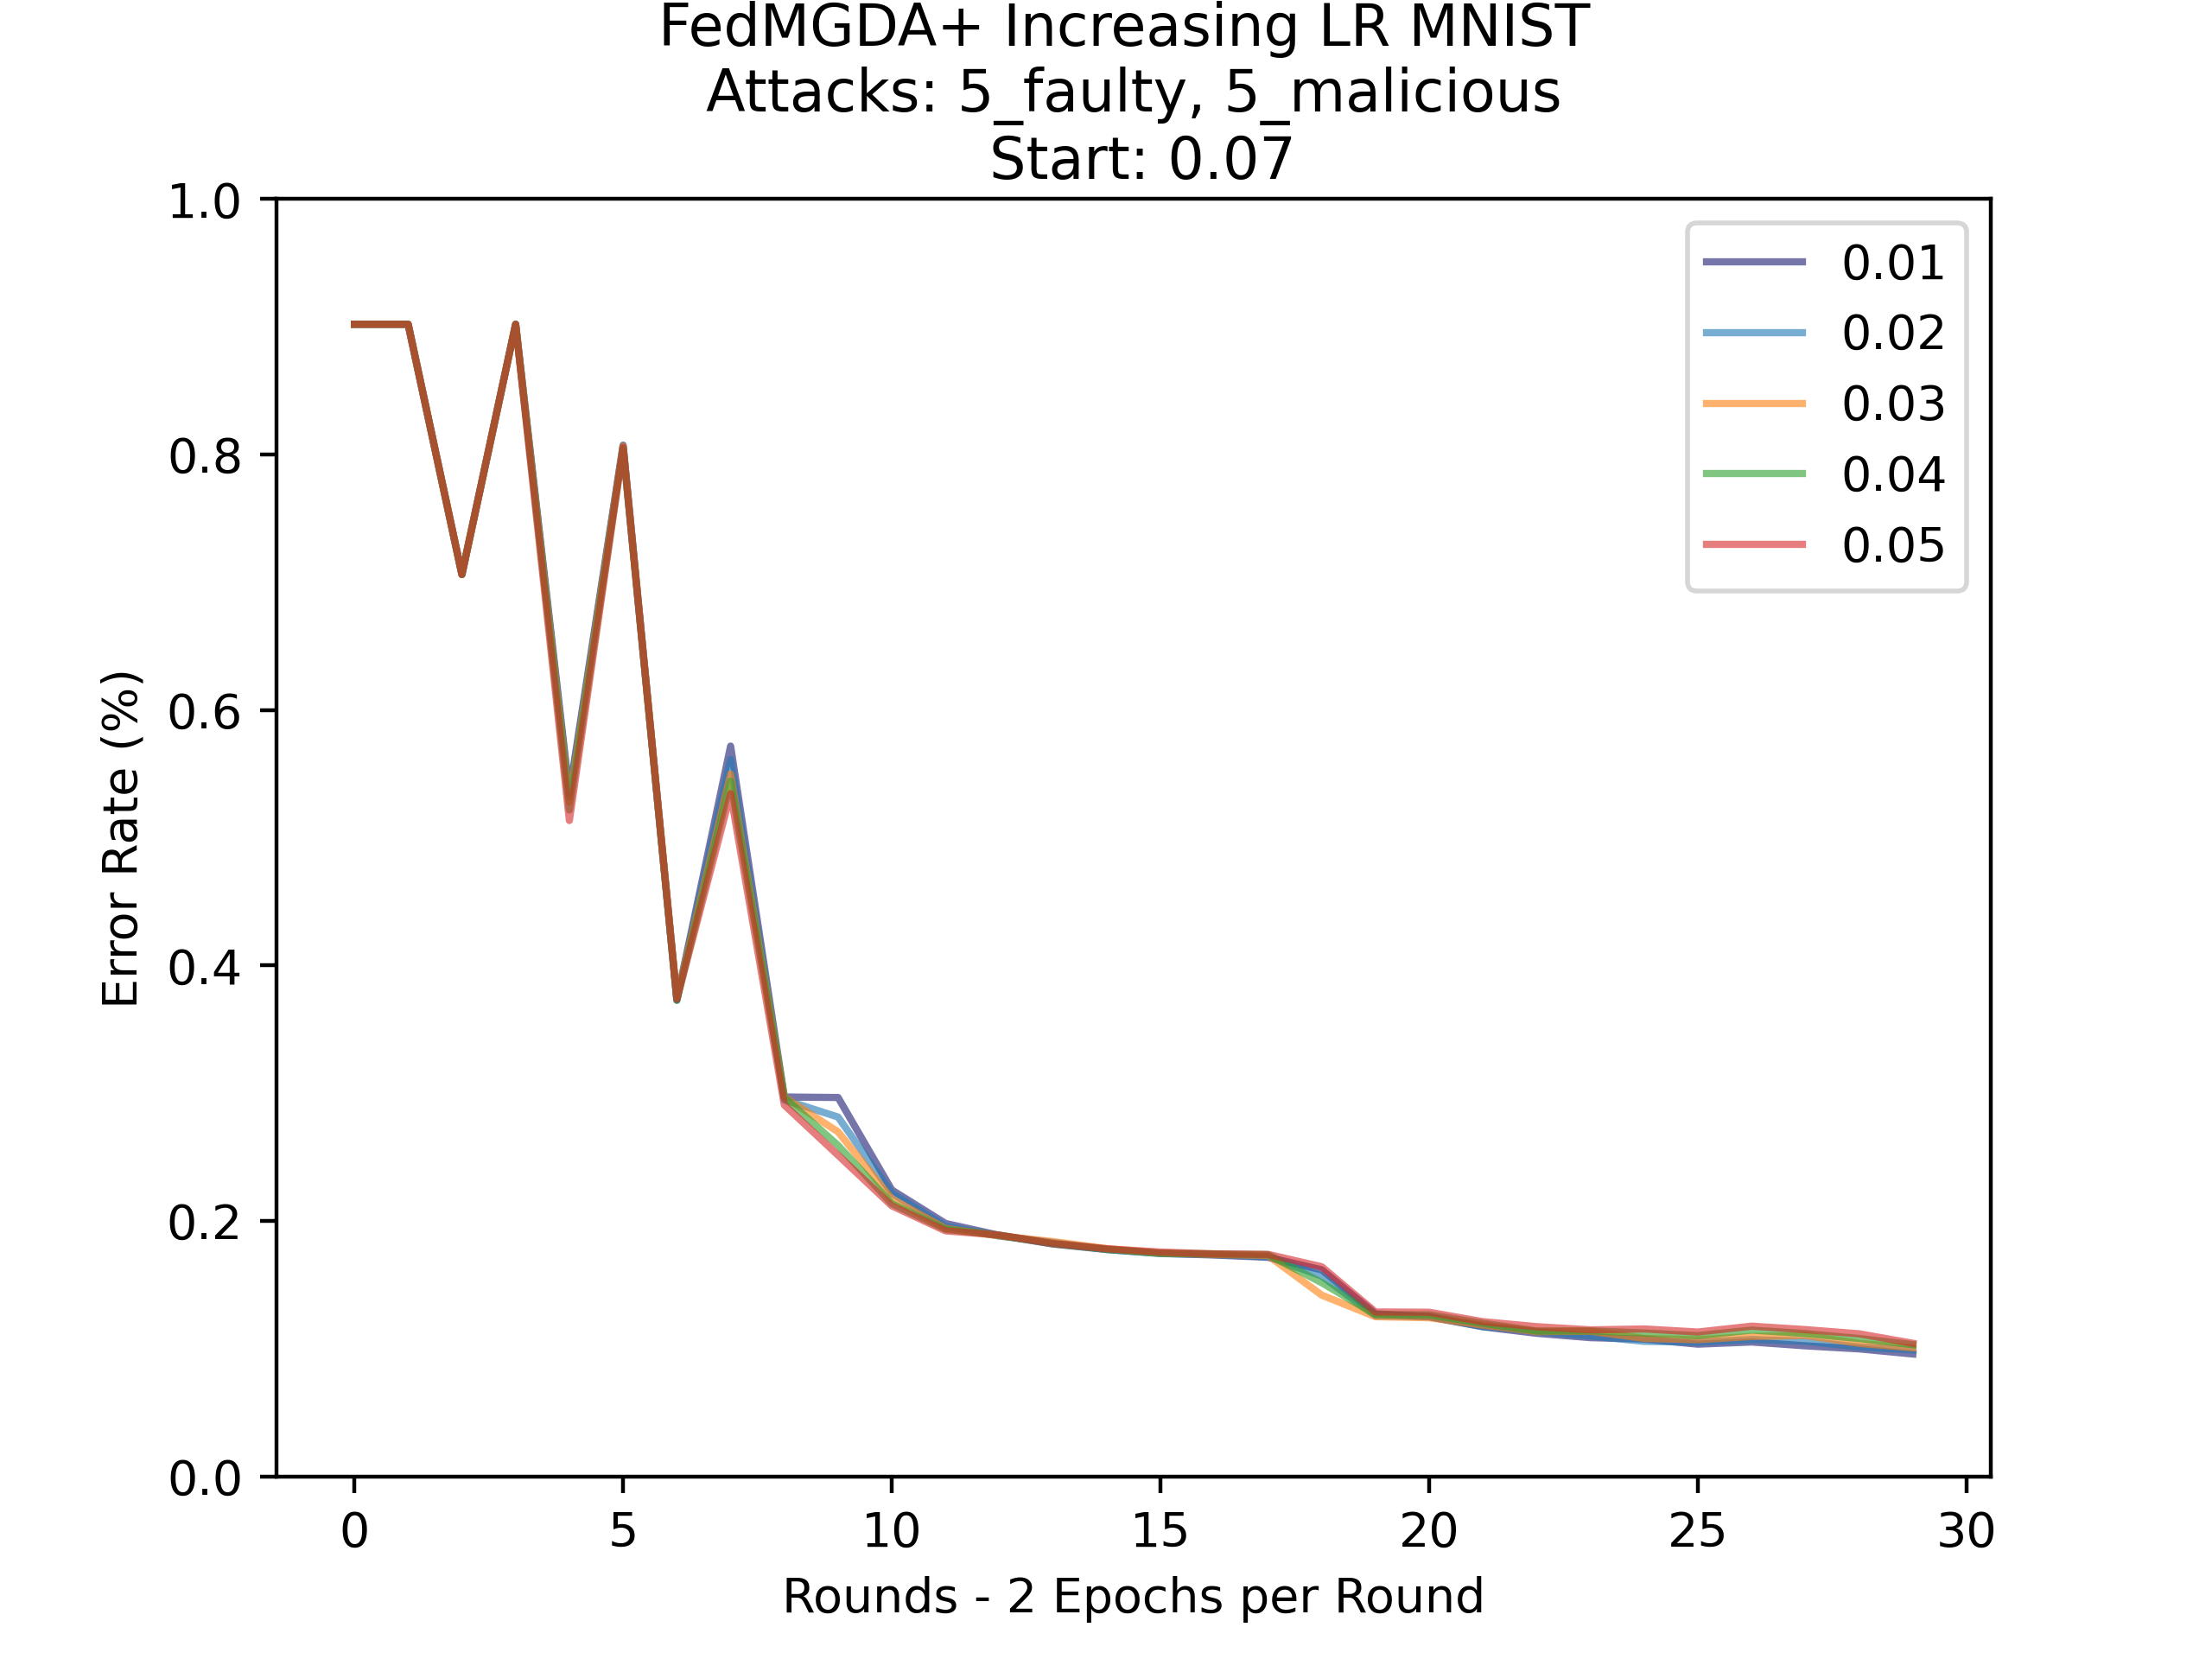
\includegraphics[scale=0.7]{initial/graphs/best_fed_result.png}
    \caption{The Error Rate graph from the best results from FedMGDA+. Notice that the performance doesn't change much but the main importance is the blocking.}
    \label{fig:best_fedmgda+}
\end{figure}

\subsubsection{Through the Looking Glass}
We now generalise our takeaways to our implementation of FedMGDA+. 
Having a more dynamic ability to vary LR will pose a greater threat to byzantine clients.
So, instead of having a fixed start and end, we have a slightly increased starting LR and now have a LR that is based on two things: when clients get blocked and when the error rate increases as opposed to decreasing.
\\ \\
This happens such that when a client gets blocked the LR decreases by a multiplier for each client that is blocked.
This allows a higher starting LR as it can quite quickly decrease once clients start to get blocked.
It also stops benign clients from getting falsely labelled later on.
Also, it is not uncommon that there is some fluctuation of the LR during federated training rounds and so having the LR increase by a set multiplier each time this happens has given some noticeable benefits as well.
It has shown greater promise in the later stages of training where the LR starts to converge but might deviate slightly.
We have seen noticeable corrections that have seemingly reduced the likelihood of late-stage benign clients being flagged as byzantine.
\\ \\
However, the performance of our model was still sub-optimal.
In attacks where only malicious clients were present, sometimes next to no malicious clients were being blocked.
Even on certain combinations of faulty \& malicious attacks, the clients would just start classifying way too many benign clients as byzantine later on.
This caused such poor performance that other weaker aggregators like MKRUM were out-performing it.
\\ \\
Another improvement made was to devise a standard deviation (std)-based approach where if the clients fell below a given threshold that would be two StDs from the mean then it would get blocked.
This was done after noticing that it was quite common for the weights of the model to look something akin to [8, 8, 9, 7, 10, \textbf{2}, \textbf{3}, 7, 6, 8, \textbf{1}].
Here the boldened numbers show weights of malicious clients that are very obviously malicious to our eyes but aren't being picked up due to not being negative or getting too low at all.
However, as seems commonplace at this point, an adaptive approach was needed.
When we tried keeping it static, depending on the attack, either clients would not be getting blocked when they needed to be, or too many benign clients would be getting blocked unnecessarily. 
We took a very similar approach to the LR in that when clients got blocked, we increased the multiple of the number of StDs from the mean that it would take before a client got blocked and we decreased the std multiplier whenever the error increased.
\\ \\
This significantly improved the algorithm. While there were still certain attacks that worked better with aggregators like COMED and AFA, Most malicious clients were now getting blocked at a frequency on-par or exceeding that of AFA.
Rather aptly, I dubbed this new method FedMGDA++.
The comparison between the old and the new method is shown below:
\begin{figure}[htbp]
    \centering
    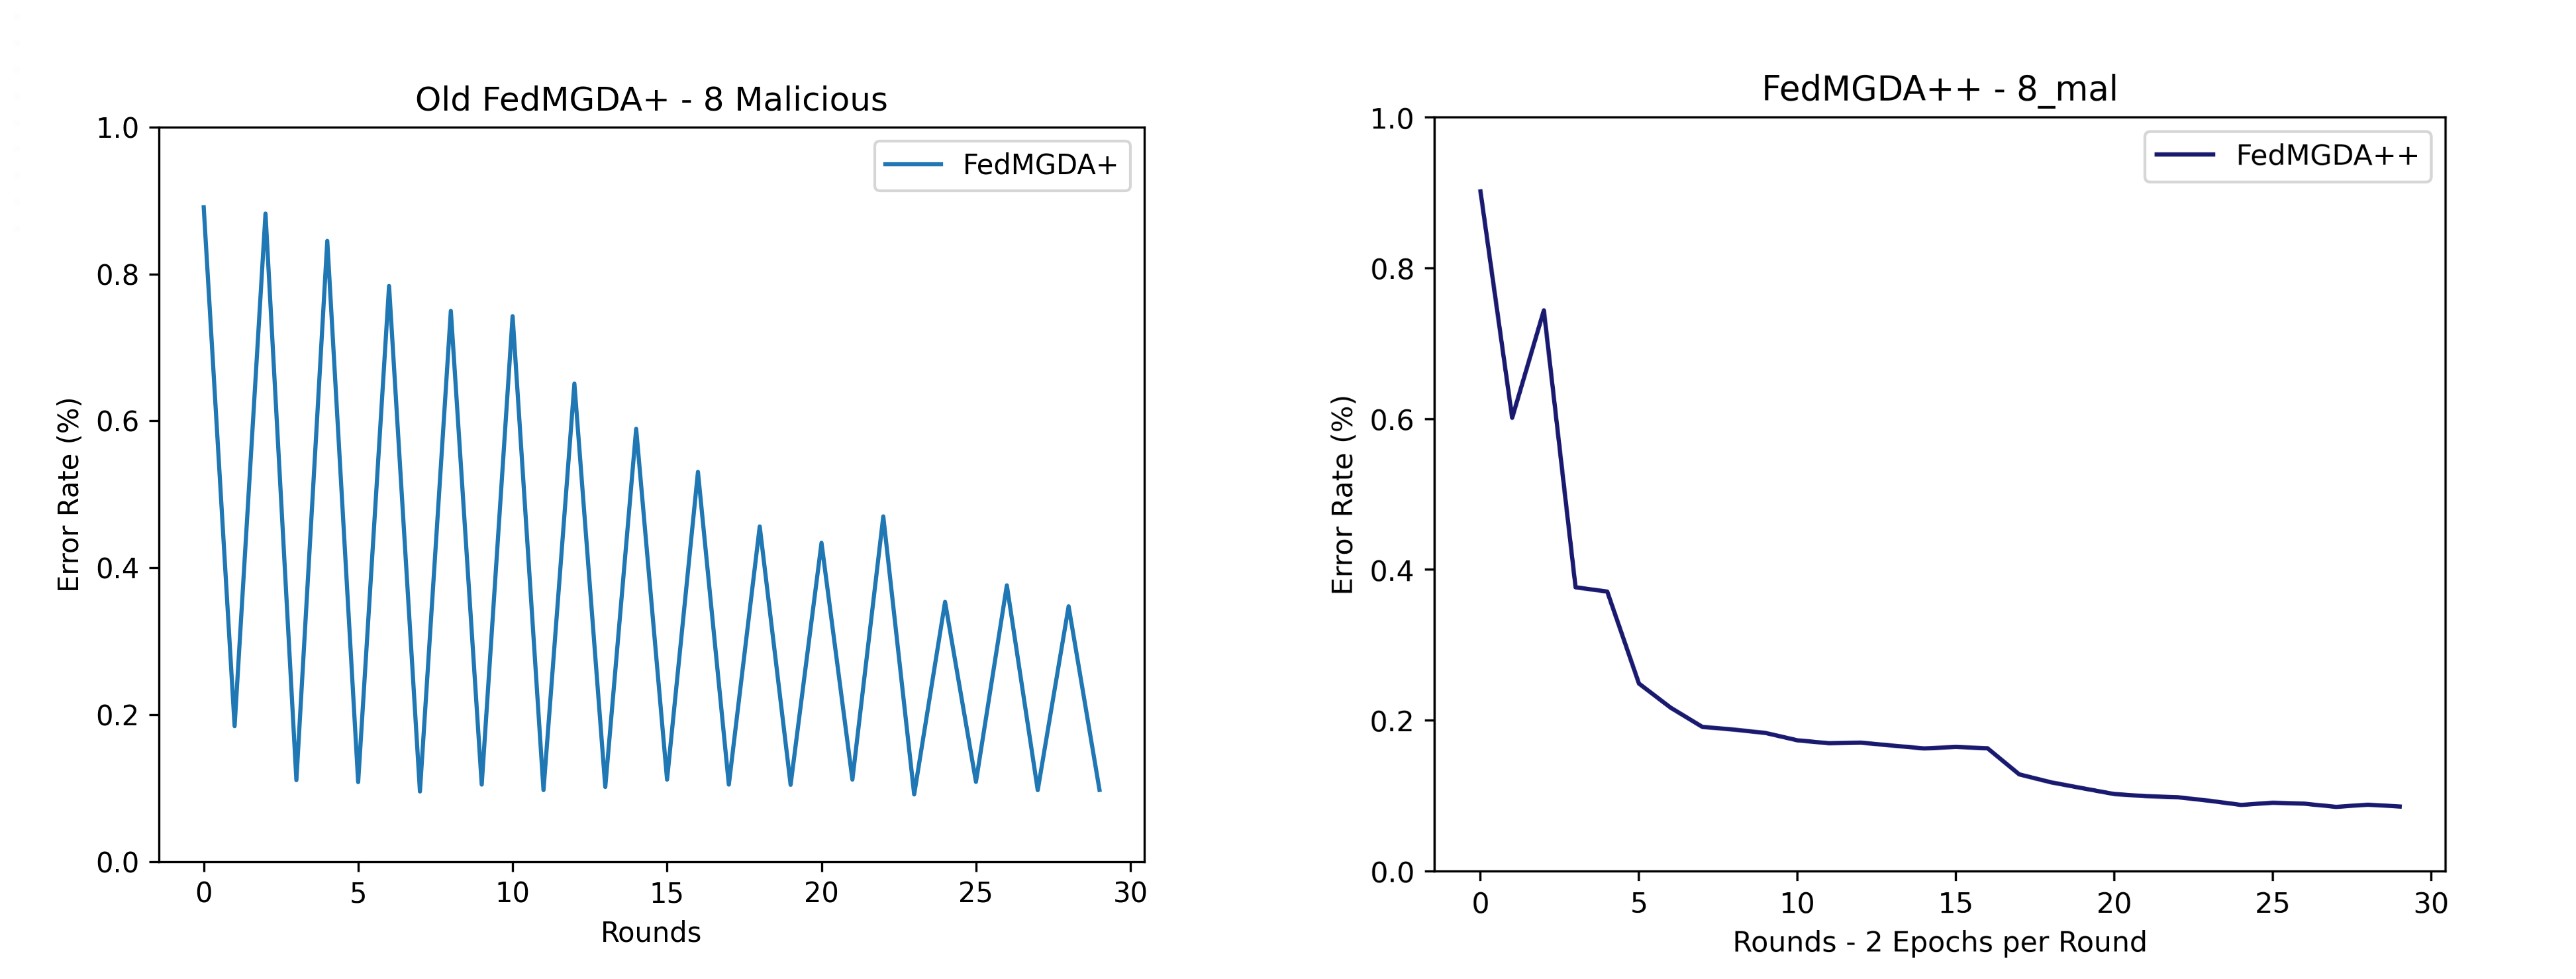
\includegraphics[scale=0.12]{initial/graphs/fedmgda_comp.png}
    \caption{Comparison between the old FedMGDA+ and the new and improved FedMGDA++ with 8 Malicious Clients with MNIST}
    \label{fig:fedmgda_comp}
\end{figure}

\section{Limitations of Robust Aggregators}
Figuring out where the aggregators thrive and where they fall short is quite crucial to determining their relevant applications or whether or not they should be used in the first place.
So, I went out to see how far the aggregators could be pushed before they either stopped learning or when too many benign clients became blocked.
We used an extreme test case of 15 faulty, 15 malicious or 10 faulty \& 10 malicious clients in the tests, to best demonstrate the aggregator's performance.


\subsection{Malicious Clients}
The first aggregator to fall comes at the five-seven malicious client mark and that is FedAvg.
It mainly starts with a performance degradation [\ref{fig:6mal}] until it simply is no longer able to learn anything of importance.
At this point both AFA and FedMGDA++ are still blocking all of the clients within the first 5 rounds.
All of the other aggregators are not noticing any performance degradation of any sort.
\\ \\
After that not much happens until the 11-12 malicious client point.
Here, AFA is the first to go [\ref{fig:11mal}] with FedMGDA++ and MKRUM not too far behind.
What is most interesting is that AFA is still fully able to recognise all of the malicious clients.
However, it does take up to the 20\textsuperscript{th} federated round before all of them are blocked.
Compare this with FedMGDA++ at round 12 and it becomes more clear to see as to why AFA starts to fail earlier.
\\ \\
\begin{figure}[htbp]
	\centering
    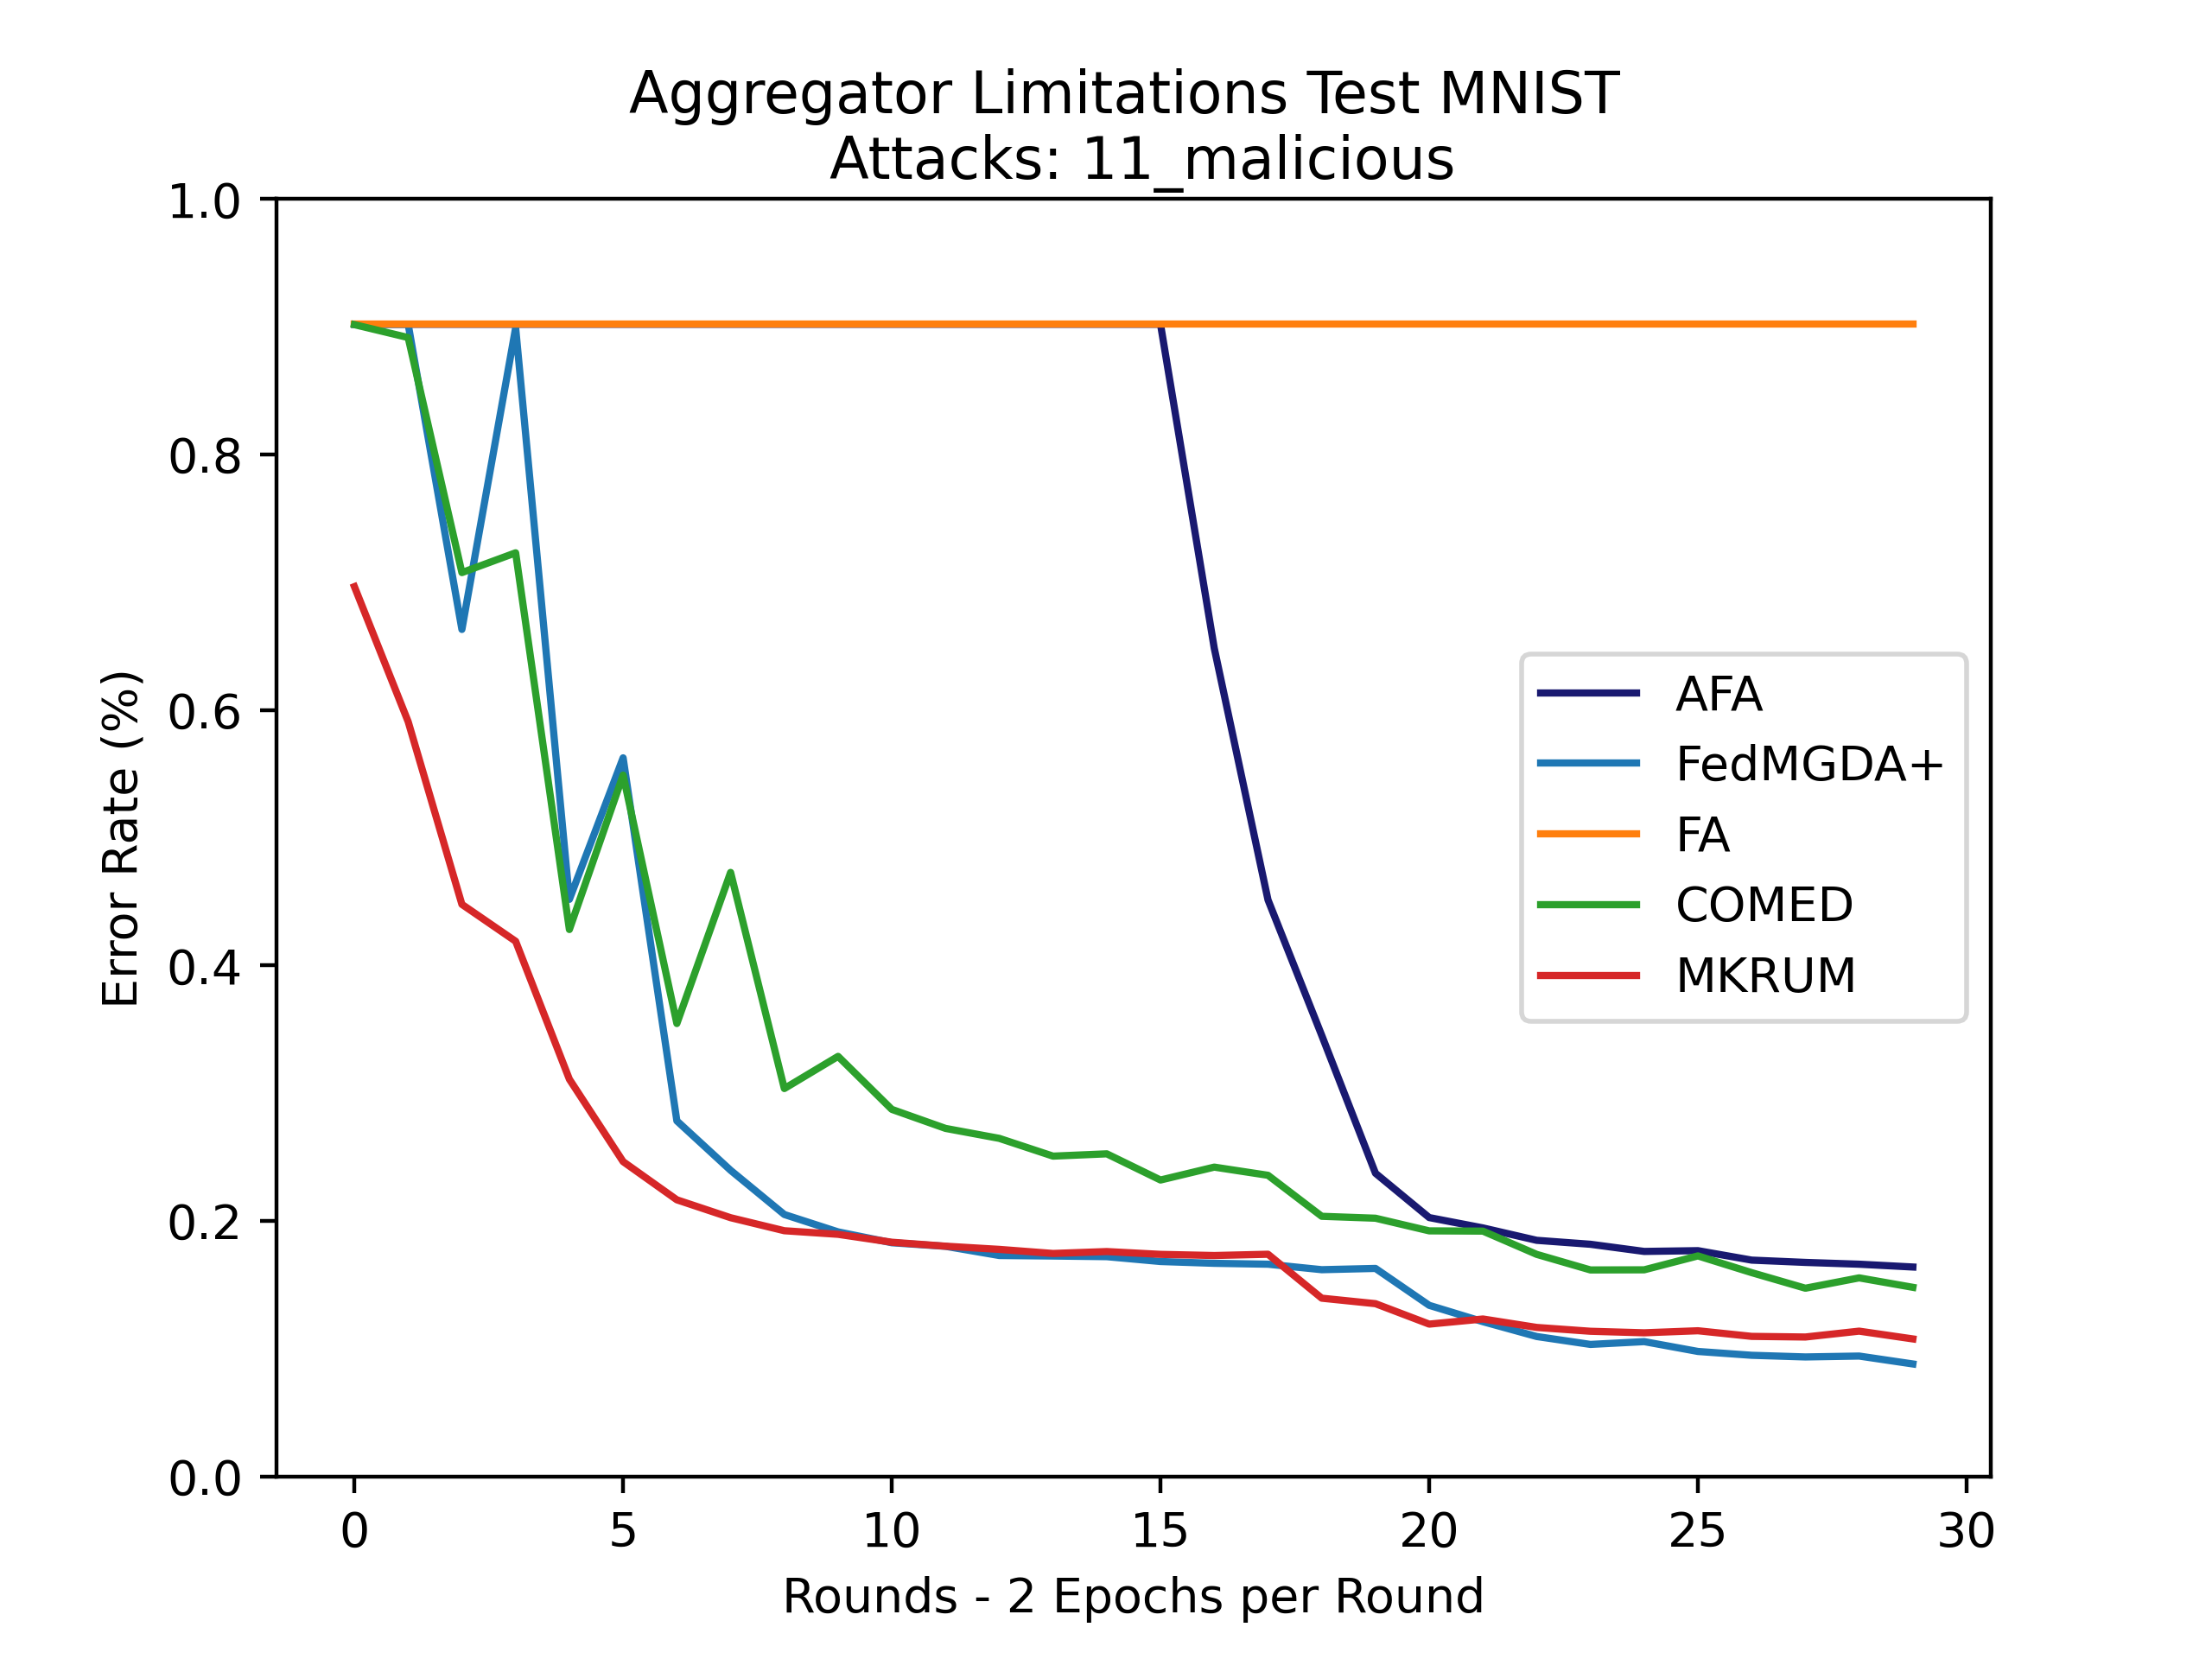
\includegraphics[scale=0.7]{initial/graphs/11_malicious.png}
	\caption{The Beginning of the End for Robust Aggregators with Malicious Clients}
	\label{fig:11mal}
\end{figure}

\\ \\
COMED ends up being the last survivor but slowly has reduced performance (down to around 60\% accuracy) before failing to learn at all.
This happens at the 15 malicious client mark which is pretty much where you would expect to see a median based solution stop being effective.
\\ \\
Something that has place for future research work is how FedMGDA++ is able to still block the majority of malicious clients while not really blocking any benign ones in the process.
This happens until even 15 malicious clients are present and shows its true testament for malicious client detection, even if it has bad performance.
Where future research can really strive is testing out how well a system in which the model is trained once with a robust aggregator with blocking, and then again afterwards without all of the blocked clients.
We believe this to have potential to allow systems that have too many malicious clients to still have the benign clients get a good model at the end of the day.


\subsection{Faulty Clients}
Immediately, FedAvg gets taken out and is not able to handle any faulty clients at all.
Very interestingly though, FedMGDA++ is the next to fall at around seven faulty clients.
What is interesting here is that it takes until about 11 faulty clients before it is completely lost.
It still shows signs and promise of learning at seven [\ref{fig:7faulty}] but just very slowly.
Similarly to with malicious clients, FedMGDA++ is still fully able to block all of the clients all of the way until the end of test at 15 faulty, past when AFA stops being able to.
\\ \\
Speaking of AFA, that is the next to go at 12 faulty clients while COMED is the only survivor even with 15 faulty.
AFA only lasts until about round 14 with the blocking but even then, it is not even blocking all of the faulty clients.
Noticeably, faulty clients are much easier to detect it seems, but they also have far more damaging effects on the model as a whole much earlier on.
\\ \\
Something that was surprising was how when the aggregators stopped being able to work properly, they weren't just forming straight lines as with malicious clients.
Instead, the accuracy was a bit rough and oscillated [\ref{fig:15faulty}], as if there was still some attempt from the model to learn but it just got overwhelmed.


\subsection{Combined Attacks}
Combined, there was nothing extra special about it.
Generally the effects felt were pretty consistent to the previous ones or a combination.
The main interesting part was that at around a combination of six malicious and six faulty, AFA and FedMGDA++ started to stop being able to recognise malicious clients as well.
As the number increased, fewer and fewer got recognised until just the faulty ones got recognised.

\section{Conclusion}
Robust aggregation has a lot of potential and a lot of different methods exist for attempting it.
What caught me off-guard the most was how well COMED did throughout.
It repeatedly was the last one standing and was able to consistently achieve good accuracy.
It really highlighted to importance of a good strategy and what it can accomplish when the applied to the correct problem.
Especially as it is becoming more common to simply slap ML on something and call it a day (\textbf{cough} FedMGDA+), it is important to reason about the problem more logically.
This is something that I aimed to do when I improved upon it and it really showed in the end.
\\ \\
One important thing to note is that while comparing Aggregators, they are not all competing for the same goal.
COMED and MKRUM both don't aim to block malicious clients and as such don't have that more complex overhead of trying to do so correctly.
So, even though it looks as if something like COMED outperforms all others, you could argue that it not blocking any clients means that it isn't on the same level as AFA and FedMGDA++.
Ultimately, it is down to personal preference with how you want to deal with the byzantine clients but it is something to note when deciding on the aggregation strategy.